

\subsubsection*{Initialize parameters from scratch} \label{sec:from_scratch}
 
In the previous examples we opened the root system parameters from an xml file. In this example we show how to do everything in a Python script without the need of any parameter file. This is especially important if we want to modify parameters in our scripts (e.g. like it is needed for a sensitivity analysis, see Section \ref{ssec:sensitivity}).

In order to set up a simulation by hand, we have to define all relevant model parameters. This is done by creating a RootRandomParameter object for each root order or root type, and one SeedRandomParameter for each plant type. 

Note that during the simulation, the parameters for a specific root (RootSpecificParameter) are generated from the RootRandomParameter class which represents the random distributions of certain parameters.

\lstinputlisting[language=Python, caption=Example 2a]{examples/example2a_initializeparams.py}

\begin{itemize}
\item[5] Matplotlib is Python's easy way to create figures like in Matlab.\item[6] NumPy is Python's scientific computing package.

\item[9,10] Create the root type parameters of type 1 and type 2.
\item[12-38] We set up a simple root system by hand. First we define the tap root L12-L26, then the laterals L28-L38. By default all standard deviations are 0. Most parameters standard deviations can be set with an additional 's' appended to the parameter name, e.g. $lmaxs$ is the standard deviation of $lmax$, see L32
\item[40,41] Set the root type parameters.

\item[43-47] Create an object of class SeedRandomParameter which defines when basal and shoot borne roots emerge. In this example we neglect basal and shoot borne roots, and just define the seed location, and deactivate basal roots by setting their maximal number $maxB$ to 0 ($firstB$ and $delayB$ are ignored in that case). 
\item[48] Sets the root system parameters.

\item[53] We choose the simulation times in a way that we can see the temporal development, and that all lateral roots have emerged in the final time step.

\item[54-70] Within the simulation loop we create Figure \ref{fig:ip}. L58-61 defines the limits and titles. In L63 we retrieve the roots as polylines which are represented by a list of nodes. In L64-67 we plot the $x$ and $z$ coordinates for each segment ($n$, $n2$) as green line. 

\item[75-80] It is not only possible to set all model parameter, 
but to retrieve the parameters after the simulation with rs.getParameter(), which returns one value per root. For all parameters that are derived from a random distribution the root specific parameter is returned (e.g. $la$, L78), i.e. the values that were drawn from the normal distribution. The root random parameter can be accessed by adding '\_mean', '\_dev' to the parameter value (e.g. $la\_mean$, L79).

\end{itemize}

Note that all parameters can be set and modified within Python. Especially, standard deviations can be set to zero in order to be able to precisely predict the result. For example we can calculate the total root system length analytically, and check if the numerical simulation yield the (exact) same result. This is performed in the tests test\_root.py, and test\_rootsystem, which is used to test and validate CPlantBox (see folder CPlantBox/test).

With such simple simulations, we can quickly check if the model does, what we expect. For example the maximal number of laterals of above parameters is 16 
$= round(lmax - la - lb)/l_n +  1$. We can calculate the time when the final lateral emerges as $-(lmax/r)*\ln(1-(lmax-l_n/2)/lmax)$ = 122.8 days. At simulation time 125 the last lateral root that has emerged is 2.2 days old, and therefore approximately 4.4 cm long (initial growth rate $r_1 = 2$), which agrees with Figure \ref{fig:ip}.

By default the length of the apical zone is fixed, when the root is created. During growth the apical zone stays in the interval $[la - l_n/2, la+l_n/2]$. The first branch emerges at length $lb$, when the root length reaches $lb +la$.

In the following two subsections we show, how tropism parameters and inter lateral spacing will affect the resulting root system.

% \begin{figure}
% \centering
% 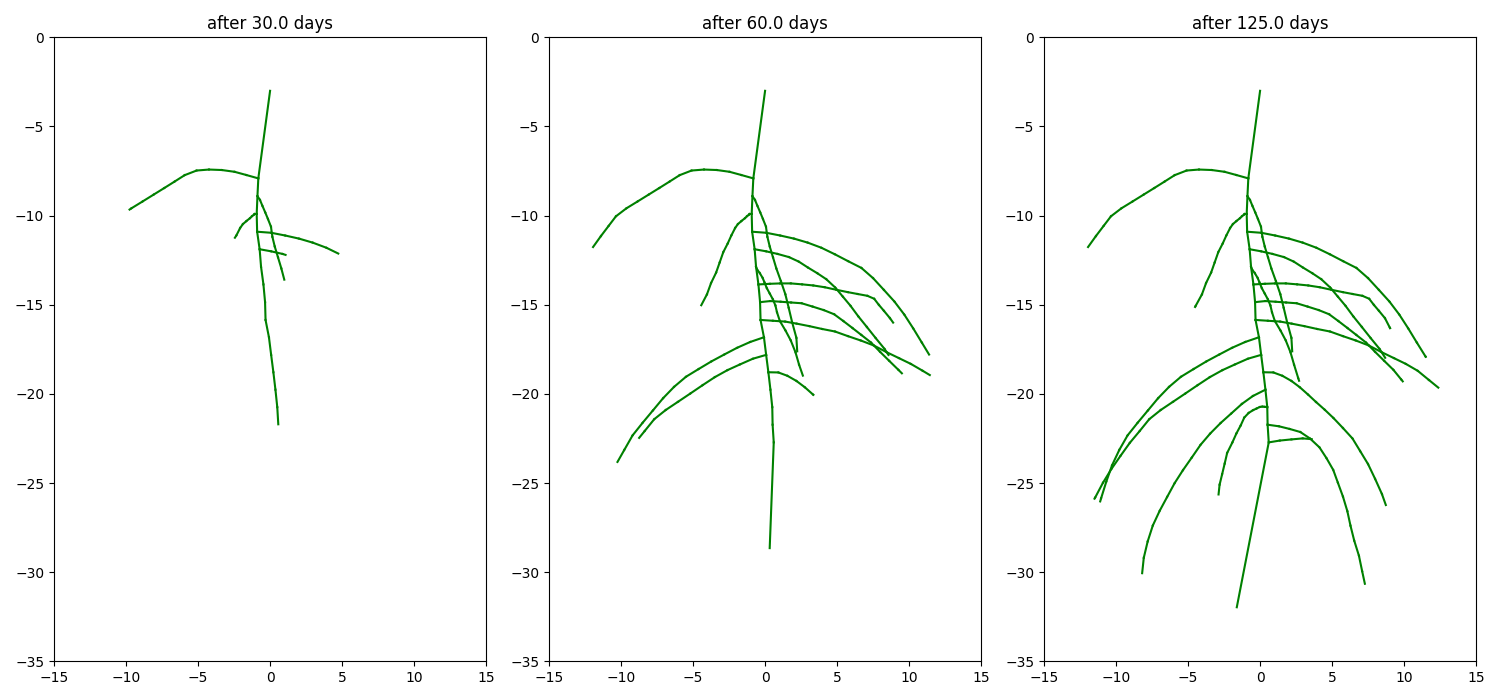
\includegraphics[width=\textwidth]{fig_initializeparams.png}
% \caption{Root development} \label{fig:ip}
% \end{figure}

\subsubsection*{Root tropism parameters $N$ and $\sigma$} \label{ssec:tropism}

We show the influence of the parameters $N$ and $\sigma$ in the case of gravitropism. The parameter $N$ [1] denotes the strength of the tropism, and $\sigma$ [cm$^{-1}$] the flexibility of the root, i.e. the expected angular variation per cm root length. 

\lstinputlisting[language=Python, caption=Example 2b]{examples/example2b_tropism.py}

\begin{itemize}
\item[10-13] We choose the parameter values $N$ and $\sigma$ we want to plot. It might be interesting to change the initial insertion $angle$, and the axial resolution $dx$. Note that a change in axial resolution should not qualitatively change the resulting images.

\item[15-18] The root system is created and SeedRandomParameters are set to produce a basal root every third day. 

\item[20-23] The RootRandomParameter for tap and basal roots is defined.

\item[25-28] The loop runs over the parameters we want to modify. We create a subplot for each configuration, and start with a new root system by calling reset in L28.

\item[30-34] We set the parameters (L30,L31) and do the simulation (L33,L34)

\item[36-44] Matplotlib is used for visualization (looping over the segments is rather slow). L36 gives a list of all nodes, and L37 of all segments as two node indices. Therefore, each segment starts at node n1 and ends at node n2, as defined in L39.

\item[L48] Creates Figure \ref{fig:tropism}.
\end{itemize}

In the first column ($\sigma$=0) of Figure \ref{fig:tropism} nothing happens, because if the root has no flexibility to bend, the strength has no influence on the resulting root system. The first row ($N$=0) shows the influence of $\sigma$ only. The growth is undirected, because the strength of the gravitropism is zero. If the roots have small flexibility, they grow downwards because they initially do. 

The other subplots show different shapes of the root system. We normally derive the two parameters $N$ and $\sigma$ by visual comparison. Note that results are independent of the root axial resolution $dx$ and the temporal resolution.
% 
% \begin{figure}
% \centering
% 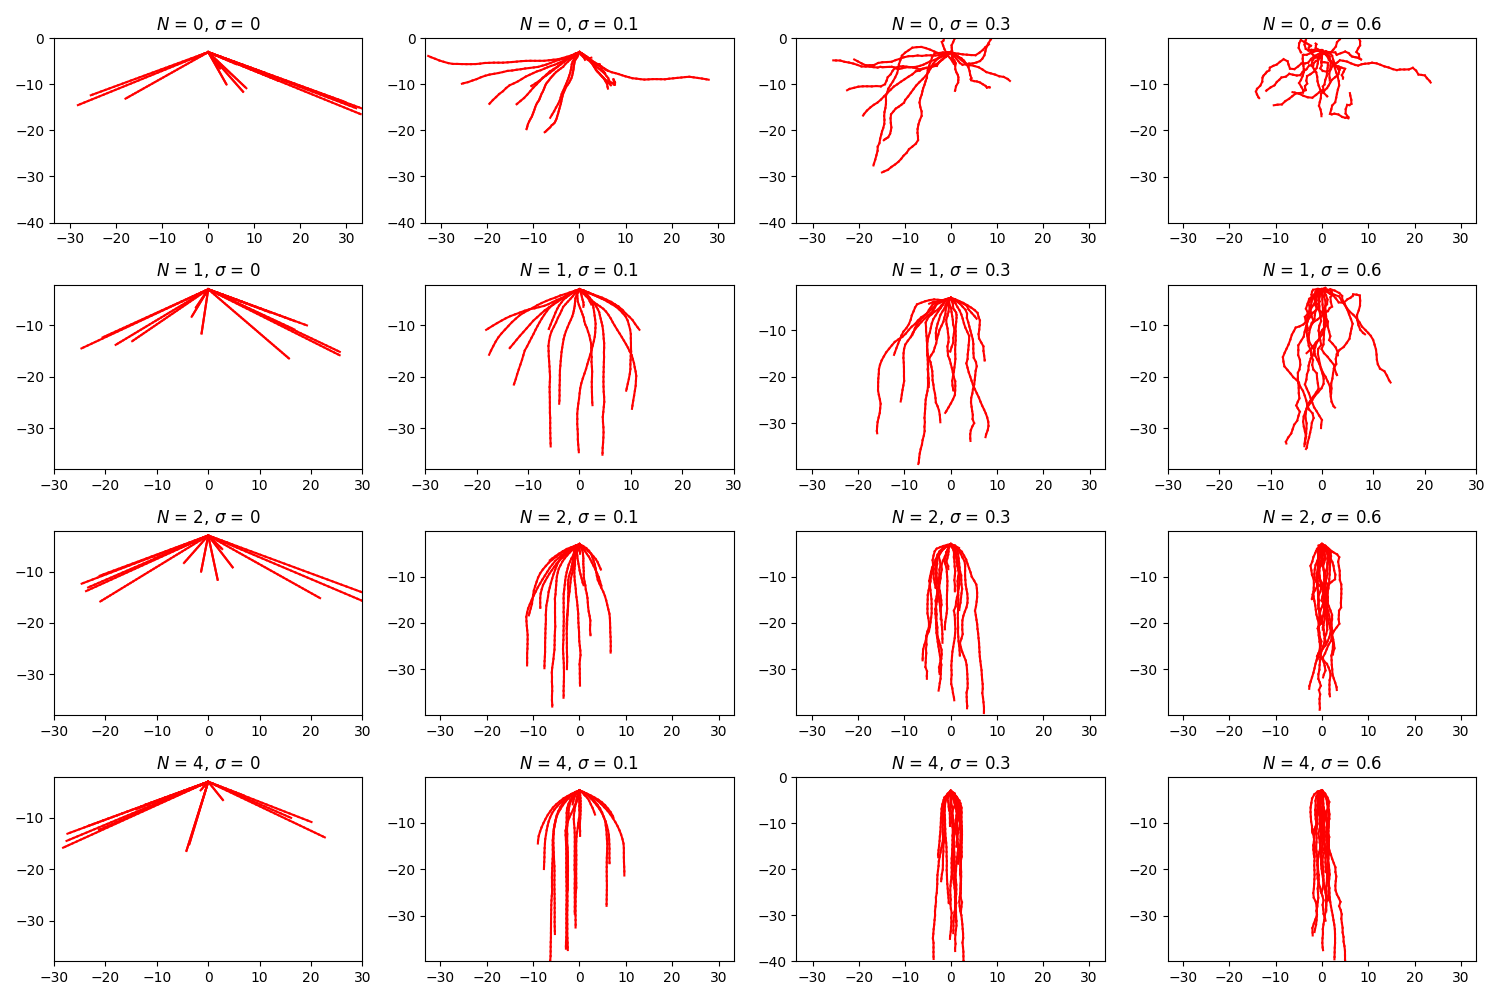
\includegraphics[width=\textwidth]{fig_gravitropism.png}
% \caption{Influence of $N$ and $\sigma$ in case of gravitropism} \label{fig:tropism}
% \end{figure}




\subsubsection*{Inter lateral spacing ($ln$, $lnk$)} \label{ssec:spacing}

A single root is divided in basal zone, root branching zone, and root apical zone. Basal and apical zone are given by the parameters $la$, and $lb$ with standard deviations $la_s$ and $lb_s$. The branching zone has the size $lmax-la-lb$, where $lmax$ is the maximal root length. The branching zone is divided into inter lateral distances $l_n$, which are values drawn from a normal distribution with standard deviation $l_{ns}$. All values are fixed when the root is created This is performed in the method RootRandomParameter::realize(). The chosen parameters reflect the root growth under perfect conditions. Based on this, the root development can then be influenced by environmental conditions e.g. impeding growth speed, or lateral emergence, see Section \ref{sec:functional}.

Normally, the setting constant branching distances is sufficient, but sometime experimental data indicate that inter lateral distances are smaller, or larger near the base than near the root tip. The reason for this could be soil root interaction (e.g. root response to dense or nutritious layer), or within the genotype. We added a purely descriptive parameter to mimic such experimental observations. The parameter $lnk$, which is zero per default, defines the slope, at the mid of the branching, altering the inter lateral distance linearly along the root axis. In the following script, we demonstrate the usage of $lnk$.

\lstinputlisting[language=Python, caption=Example 2c]{examples/example2c_lateralspacing.py}

\begin{itemize}
\item[10-13] A root system with a single tap root is created. 
\item[16,16] The axial resolution, and insertion angle is defined. We take a very large axial resolution for the tap root, since we visualize the nodes later on, and we want to see only lateral branching nodes.
\item[18-24] Definition of the tap root. Standard deviations are zero, we do not want any variations. Tropism parameters are chosen in a way, that the tap root grows straight downwards.
\item[26-29] Definition of the first order lateral. Tropism is a strict exotropism (i.e. root follows its initial growth direction).
\item[31,32] The parameter values we want to visualize.
\item[36] Resets the root system (to $simTime = 0$). Root parameters are not changed. 
\item[38,39] Sets the values for this subplot. 
\item[41,42] Runs the simulation
\item[44-56] Creates the subplots. First (L47-49) we plot all segments in green. And second (L51-53) we plot all nodes of the tap root as red asterisks.
\item[58-60] Creates Figure \ref{fig:spacing}
\end{itemize}

The mid column of Figure \ref{fig:spacing} shows to different inter lateral distances, 4 (top) and 2 (cm) bot. The left column demonstrate the use of negative values for $lnk$ which results in larger distances near the base. The right column has positive values for $lnk$, which will result in smaller distances near the base. The $i$-th inter distance is calculated as $ln_i = ln + lnk (x_i-mid_x)$, where $x_i$ is the position within the branching zone, and $mid_x$ is the mid of the branching zone. This is done in RootRandomParameter::realize(). Note that $lnk$ is dimensionless and the slope in the linear equation. At mid of the branching zone the inter-lateral distance equals $ln$. 

% \begin{figure}
% \centering
% 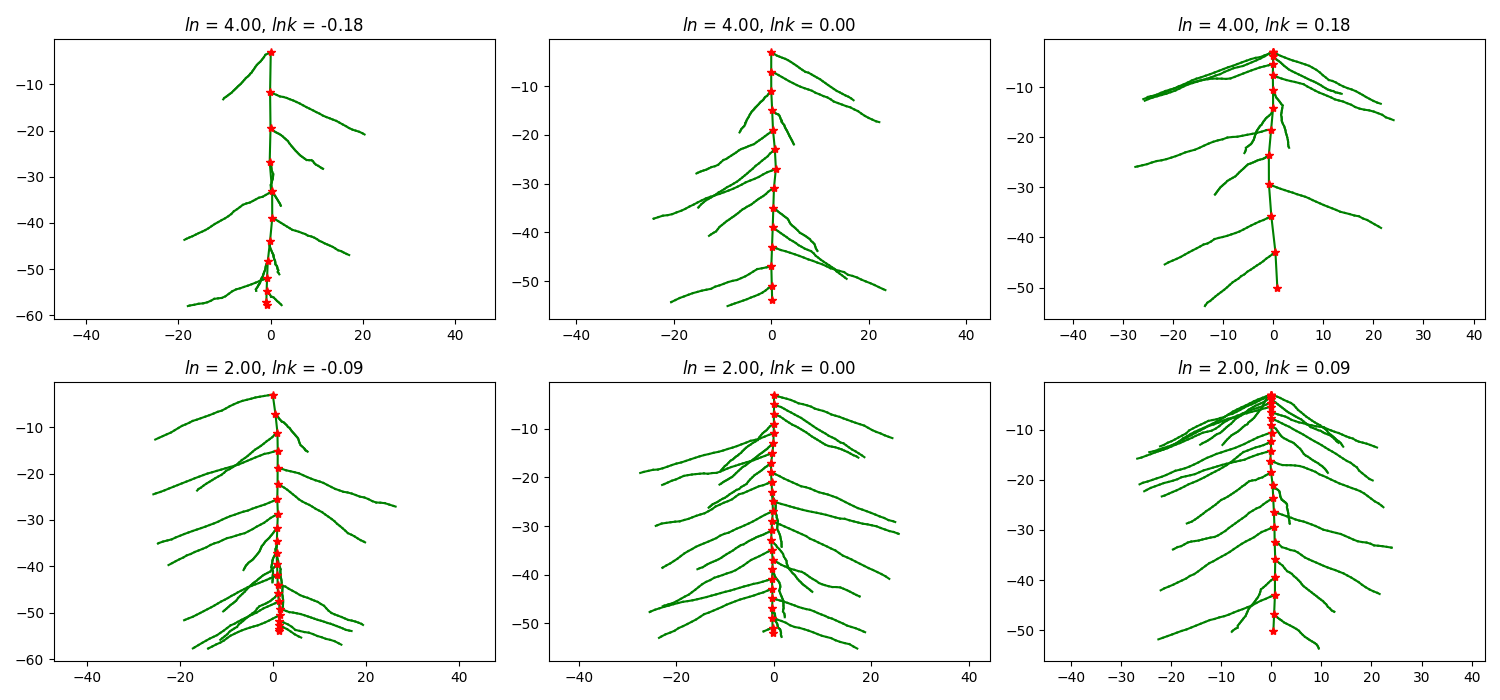
\includegraphics[width=0.99\textwidth]{fig_lateralspacing.png}
% \caption{Inter-lateral spacing, larger near base (left column), constant (mid column), and smaller near base (right column) } \label{fig:spacing}
% \end{figure}

In the following we show, how to analyse model results on a per root basis using the RootSystem class. To create density distributions the resulting root segments are analysed using the SegmentAnalyser class, described in Section \ref{sec:sa}.

\newpage
\subsubsection*{Tropisms} \label{sec:tropism}

The change in root growth direction is described by tropisms. In the following we show how to implement directed growth toward higher water content or nutrient concentration, and demonstrate how to simply make new user defined tropism rules. 


Root growth direction is influenced by soil conditions such as water content, soil strength, or nutrient concentration. In the following example we model the influence of a nutrient rich layer to root system development

\lstinputlisting[language=Python, caption=Example 4a]{examples/example4a_hydrotropism.py}

\begin{itemize}

\item[6-9] Creates the root system and opens the parameter file

\item[12-17] Change the tropism for all root types: L13 modifies the axial resolution, L14 set the tropism to hydrotropism, and L15-16 sets the two tropism parameters. The parameter $\sigma$ is set to 0.4 for the tap root ($subType$ = 1), and to 1. for the rest of the root types.

\item[19-25] Definition of a static soil property using SDF. We first define the geometry (L20-L21), and then create a static soil (L22) that obtains the maximal value $maxS$ inside the geometry, 
$minS$ outside the geometry, and linear slope with length $slope$. At the boundary the soil has the value $(maxS+minS)/2$.

\item[28] Sets the soil. Must be called before RootSystem::initialize()

\item[41] Initializes the root system, and among others sets up the hydrotropism. 

\item[33-39] Simulation loop

\item[42] Exports the root system geometry

\item[45-46] We actually do not wish to set this geometry, but we abuse the writer of the class RootSytem to export a Python script showing the layer geometry. The resulting ParaView visualization is presented in Figure \ref{fig:chemo}.

\end{itemize}

% \begin{figure}
% \centering
% 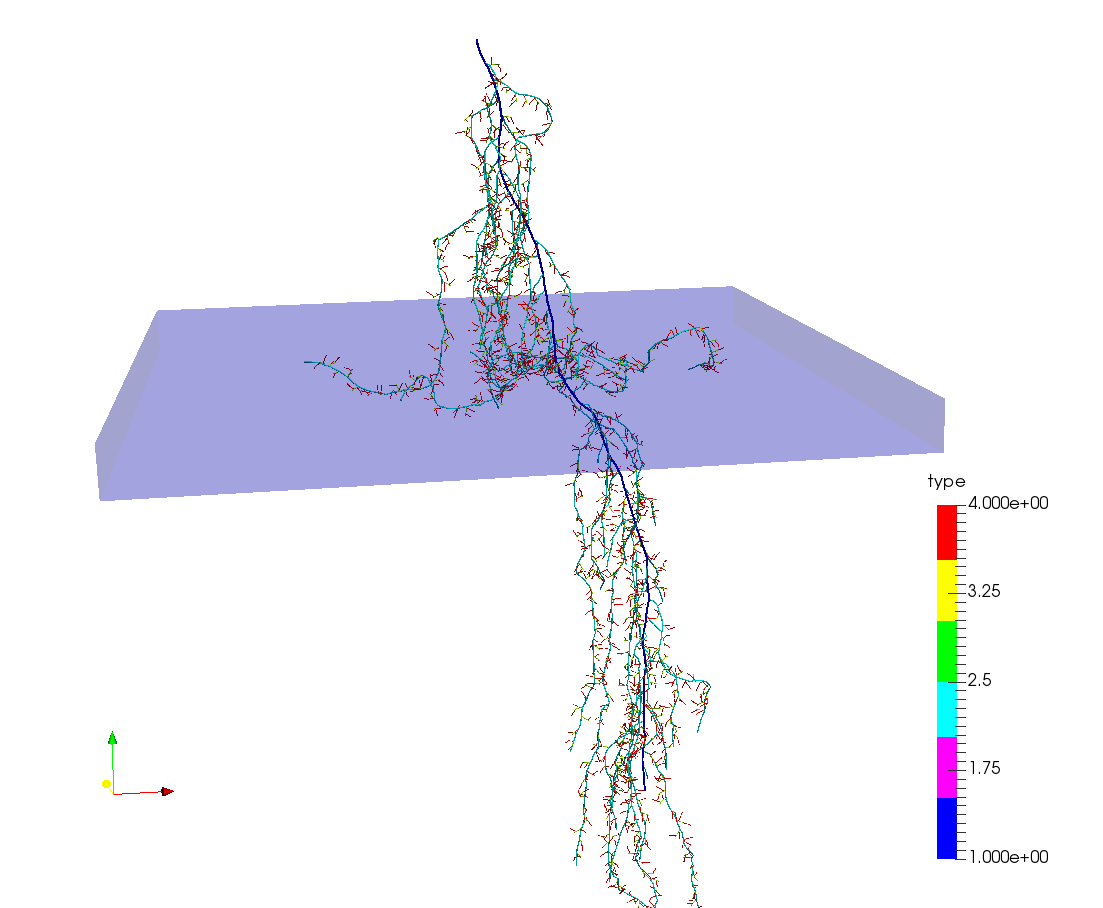
\includegraphics[width=0.7\textwidth]{example4a.png}
% \caption{Chemotropism in a nutrient rich layer (Example 4a)} \label{fig:chemo}
% \end{figure}

Normally, the simulation is created from a set of parameters. For tropisms these are the type of tropism $T$, number of trials $N$ , and tortuosity $\sigma$. There are only a few predefined tropisms called 'gravi', 'plagio', 'exo', or 'hydro', but it is simple to add user defined tropisms.
The following example demonstrates how to define a root age dependent tropism, where roots first grow according to exotropism (following the inital growth direction), and after a certain age change to gravitropic growth.

The new tropism class must be derived from the class Tropism. In CPlantBox tropism is realised with a random optimization process, where the 'best' direction is chosen from $N$ possible direction, according to an objective function that is minimized. Normally, it is sufficient to overwrite this function, called Tropism ::tropismObjective, to change the tropism behaviour. This can be done in Python or in C++. The classes Hydrotropism, Gravitropism, and Plagiotropism (in tropisms.h) are examples for this procedure.

If the whole concept of random optimization is altered, Tropism ::getUCHeading must be overwritten, which is only possible in C++. If the geometry model is also changed Tropism::getHeading must be overwritten.

The following example shows how to implement a new tropism in Python. Two new tropism are introduced:
The first does nothing but to output the incoming arguments of the method Tropism::tropismObjective to the command line (e.g. for debugging). The second one describes a root age dependent tropism that starts with exotropism and changes with root age to gravitropism.

\lstinputlisting[language=Python, caption=Example 4b]{examples/example4b_usertropism.py}

\begin{itemize}

\item[8-19] Creates a new tropism that just writes incoming arguments of Tropism ::tropismObjective to the command line. This can be used for debugging. The new class is extended from rb.Tropism, and the method Tropism ::tropismObjective is overwritten with the right number of arguments.

\item[22-37] Again, we extend the new class from rb.Tropism. In L25-30 we define our own constructor. Doing this two things are important: (a) the constructor of the super class must be called (L26), and (b) the tropism parameters $n$, and $\sigma$ must be set (L29). 
Furthermore, the constructor defines two tropisms: exo- and gravitropism, that are used in Tropism::tropismObjective at a later point, and a root age that dermines when to switch betwee exo- and gravitropism. \\
In L32-L37 the method Tropism::tropismObjective is defined. We choose the predefined objective function depending on the root age.

\item[41-45] Sets up the simulation.

\item[48-51] L48,L49 creates the first user defined tropsim. Since we did not define a constructor Tropism::setTropismParameter must be called. L50 creates the second user defined tropism.  In L51 the tropism is chosen, using the method Tropism::setTropism. The second argument states for which root type it applies. 
Number 4 is the (default) root type for basal roots, -1 states that the tropism applies for all root types (default = -1).

\item[54-58] The simulation loop. 

\item [61] Exports the result producing Figure (\ref{fig:tropism}). 

\item [64] VTK plot.

\end{itemize}

% \begin{figure}
% \centering
% 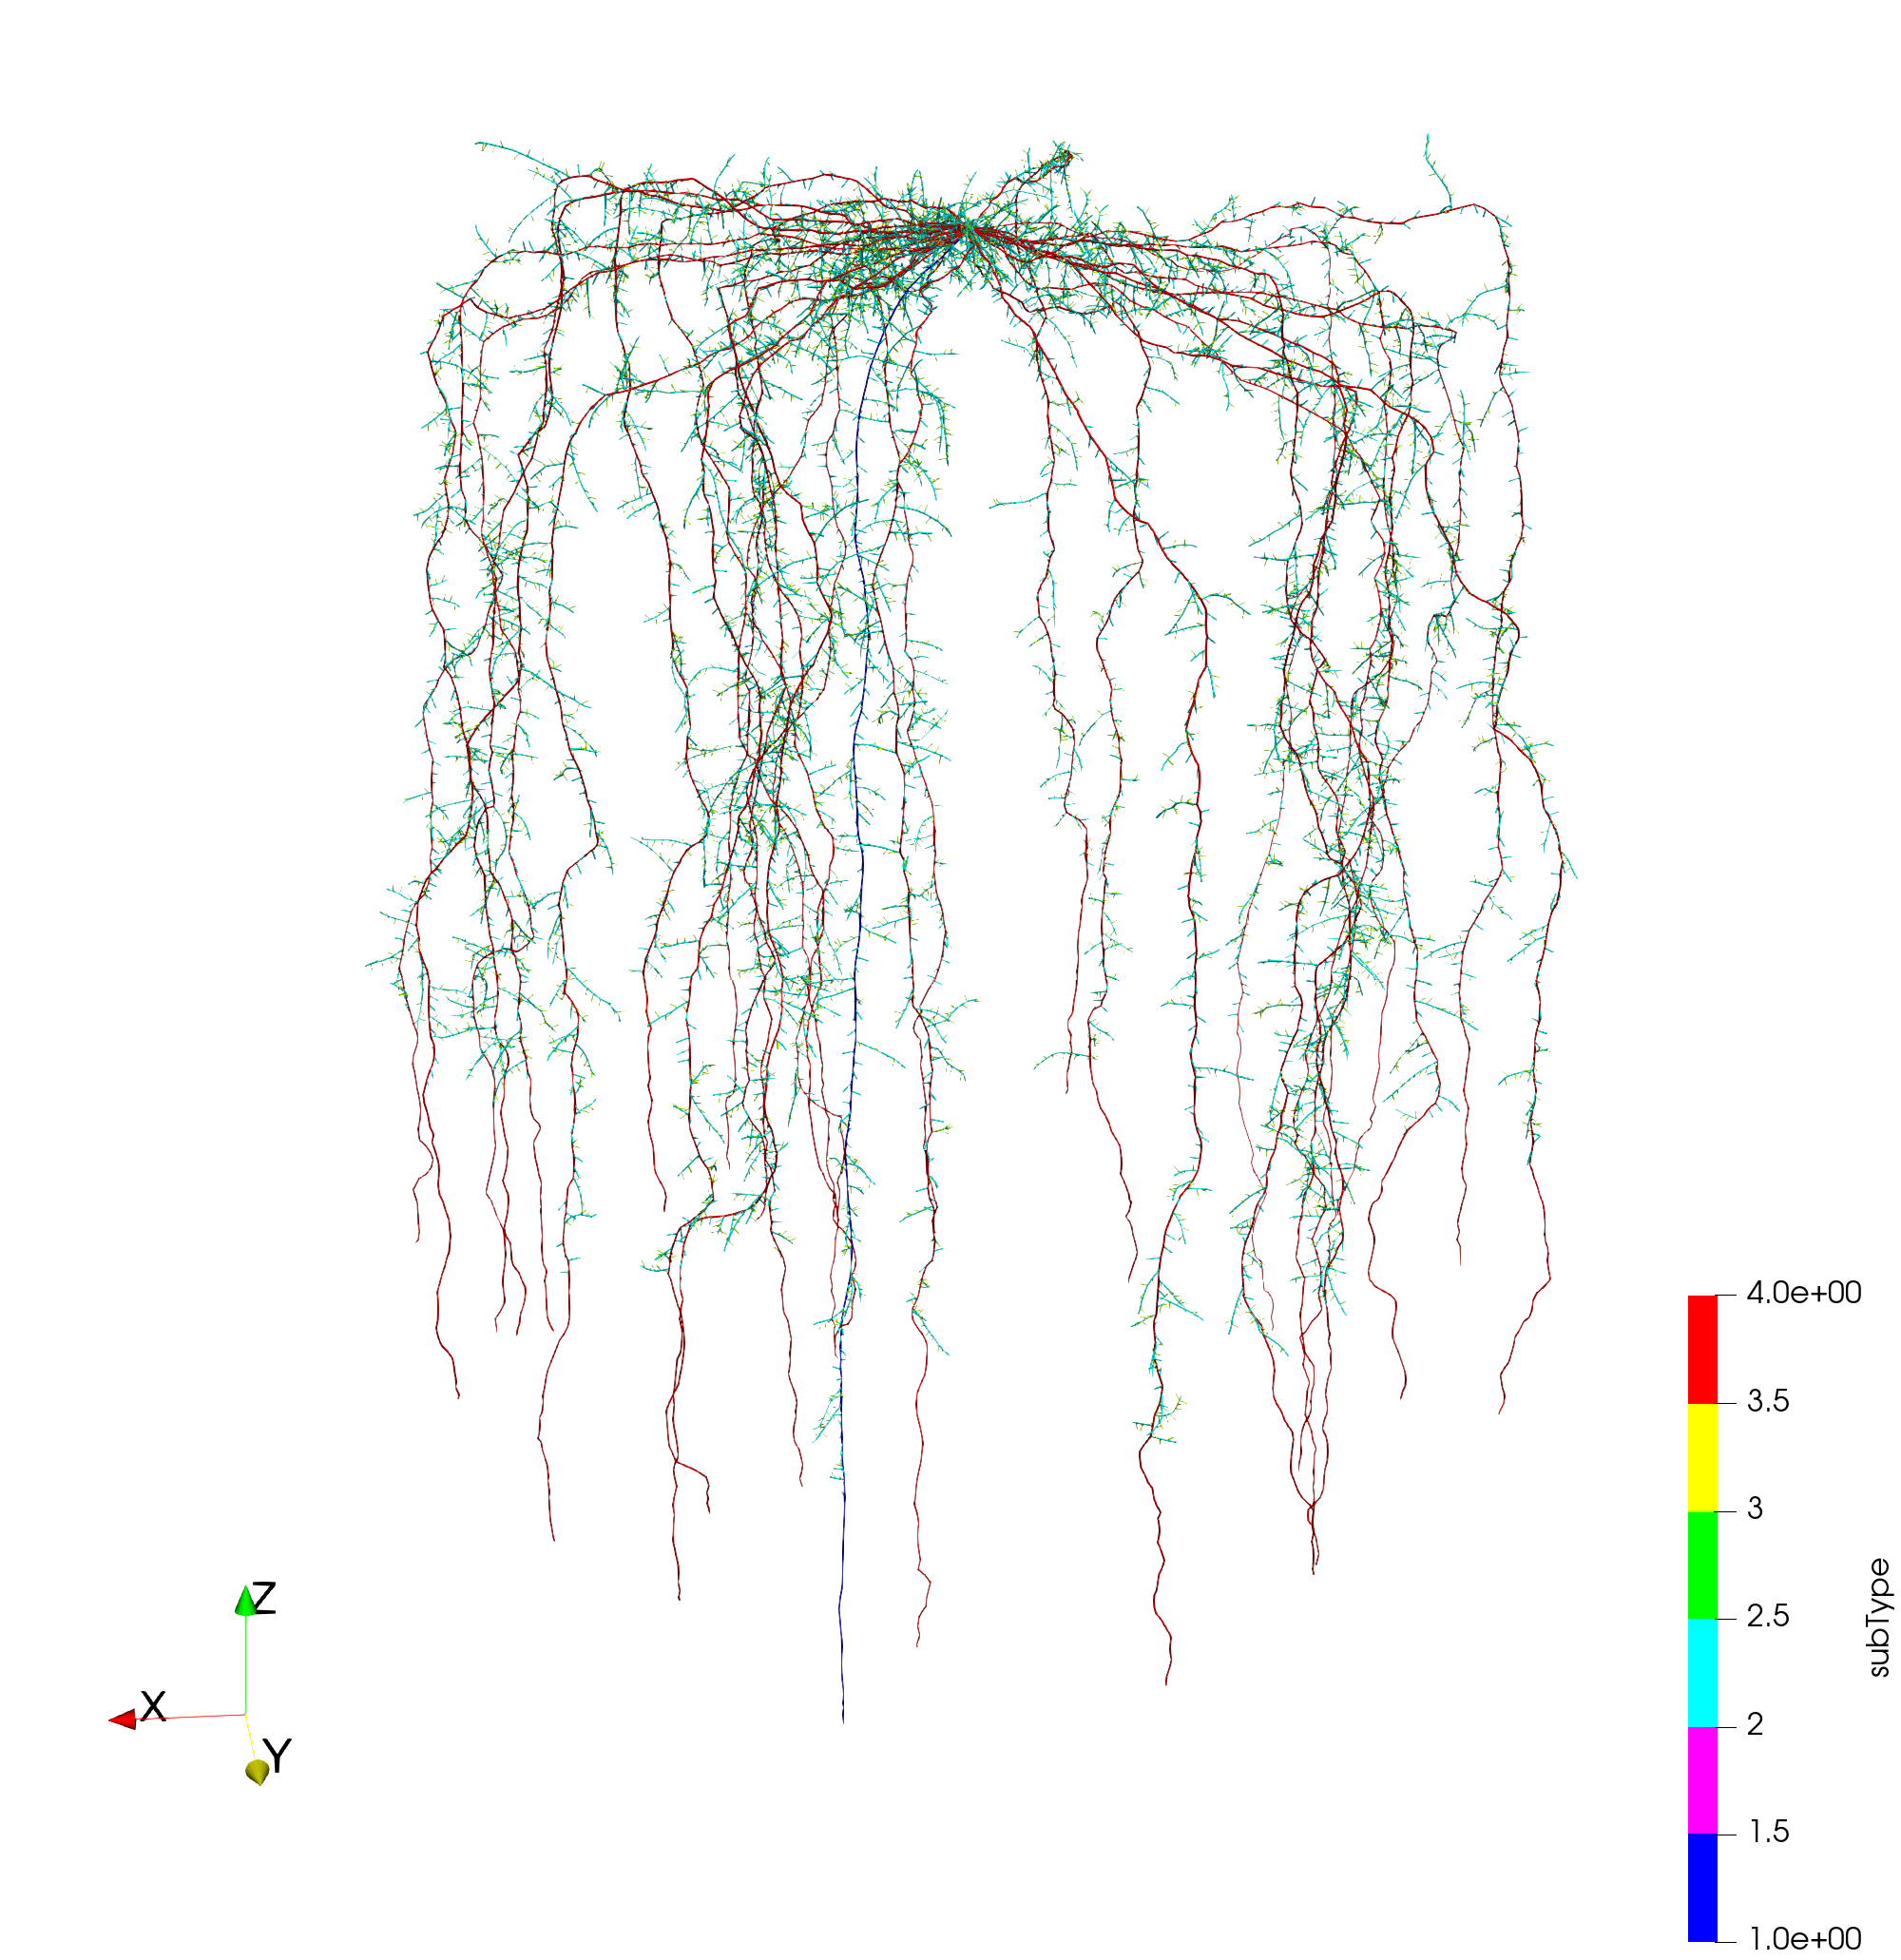
\includegraphics[width=0.7\textwidth]{example4b.png}
% \caption{Depending on root age the laterals follow plagio- or gravitropism (Example 4b)} \label{fig:tropism}
% \end{figure}




